\section{多目标优化}
\label{sec:opt-mmb-multiobjective}

本节处理多个指标同时要求变小的问题，即\term{多目标优化}（multiobjective optimization）。标量优化中任意两个候选都能比较大小；指标变成向量之后，有些候选之间无法比较，“最优”只能先定义为“没有被全面超过”。这样留下的通常是一整批候选，要从中选出一个，还必须补充一种偏好。本节先建立比较关系与解集，再依次讨论两种表达偏好的方式——加权求和与设置阈值，最后讨论不预先给定偏好、只求同时改善全部指标的局部方法。

本节固定可行域$C\subseteq\mathbb R^d$与$m$个都要最小化的指标$f_1,\dots,f_m:C\to\mathbb R$，记$\bm f=(f_1,\dots,f_m)$。这里的$m$是指标个数，与约束个数无关。

\subsection{支配与Pareto最优}
\label{sec:opt-mmb-pareto}

\paragraph{一个有限候选例}
设我们要从六个候选模型中选一个部署，每个模型有两项指标：推理延迟$f_1$（毫秒）和验证误差$f_2$（百分点），数值是教学用的假设数据：
\begin{equation}
\label{eq:opt-mmb-six-candidates}
\begin{aligned}
&A=(1,5),\quad B=(2,2.5),\quad C=(3.5,2.2),\\
&D=(5,1),\quad E=(4,4),\quad F=(6,1).
\end{aligned}
\end{equation}
图~\ref{fig:opt-mmb-pareto-candidates}把它们画在目标平面上。$E$比$B$慢，误差也比$B$大，无论我们更在乎哪一项，都没有理由选$E$。$A$与$D$的关系则不同：$A$更快，$D$更准，单凭这两组数无法断定谁更好。比较向量时，“全面不差且至少一项更好”是唯一不依赖偏好的判断。

\begin{definition}[支配与Pareto最优]
\label{def:opt-mmb-pareto}
设$\bm u,\bm v\in C$。若$f_i(\bm u)\leq f_i(\bm v)$对所有$i$成立，且至少有一个$i$使不等号严格成立，称$\bm u$\term{支配}（dominate）$\bm v$。不被任何可行点支配的$\bm v\in C$称为\term{Pareto最优}（Pareto optimal）点；若不存在可行点$\bm u$使$f_i(\bm u)<f_i(\bm v)$对所有$i$同时成立，则称$\bm v$为\term{弱Pareto最优}（weakly Pareto optimal）点。
\end{definition}

Pareto最优点组成的集合称为Pareto集合，它位于参数空间$C$中；它在$\bm f$下的像称为\term{Pareto前沿}（Pareto front），位于目标空间$\mathbb R^m$中。Pareto最优一定弱Pareto最优，因为所有指标都严格更小的点当然支配它；反过来不成立，弱Pareto点可以被“一项相同、另一项更好”的点支配。

\begin{figure}[!htbp]
  \centering
  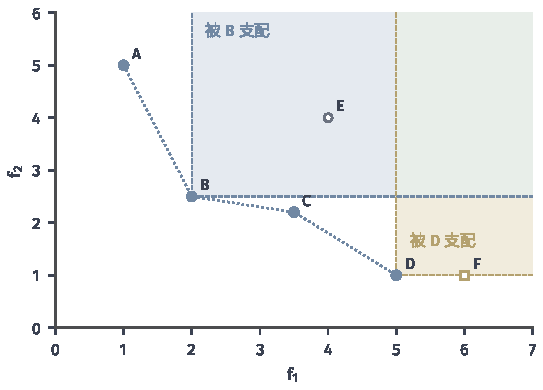
\includegraphics[width=92mm]{figures/03-optimization-evolution-and-signals/01-optimization/matplotlib/c7-pareto-candidates/figure.pdf}
  \caption{式~\eqref{eq:opt-mmb-six-candidates}中六个候选在目标平面上的位置，横轴为延迟$f_1$，纵轴为误差$f_2$。蓝色阴影是被$B$支配的区域，黄色阴影是被$D$支配的区域（重叠部分为绿色）。$E$落在$B$的阴影里；方块$F$落在$D$的阴影边界上，只与$D$误差相同而更慢，所以被支配，却仍是弱Pareto最优。实心点$A,B,C,D$构成Pareto前沿，点线只表示前沿上的顺序。}
  \label{fig:opt-mmb-pareto-candidates}
\end{figure}

\paragraph{有限例中的三类候选}
逐对核对式~\eqref{eq:opt-mmb-six-candidates}即可分类。$E$被$B$（也被$C$）支配；$F$被$D$支配。$A,B,C,D$按延迟递增排列时误差严格递减$5>2.5>2.2>1$，任意两者都是一项更好、一项更差，又不被$E,F$支配，所以都是Pareto最优点。$F$的情形值得注意：要找到两项都严格小于$F=(6,1)$的候选，需要误差小于$1$，而没有候选做到这一点，所以$F$是弱Pareto最优的，尽管它被$D$支配。后面比较各种选择方法时，都以这六个候选为共同对象。

\paragraph{参数空间与目标空间}
连续问题中，Pareto集合与前沿通常是曲线或曲面，二者不在同一个空间。取$C=\mathbb R^2$与
\begin{equation}
\label{eq:opt-mmb-two-quadratics}
f_1(\bm x)=\tfrac12\lVert\bm x-\bm a\rVert_2^2,\qquad f_2(\bm x)=\tfrac12\lVert\bm x-\bm b\rVert_2^2,\qquad \bm a=(1,0),\ \bm b=(-1,0).
\end{equation}
若$x_2\neq0$，把第二个坐标改成零会使两项同时严格减小；若$x_2=0$而$x_1>1$，点$\bm a$使$f_1$减为零、$f_2$也变小；$x_1<-1$时对称。于是只有线段$\{(s,0):-1\leq s\leq1\}$上的点可能是Pareto最优点；在这条线段上，$s$增大使$f_1=(s-1)^2/2$减小而使$f_2=(s+1)^2/2$增大，任意两点互不支配，所以Pareto集合恰是这条线段。图~\ref{fig:opt-mmb-pareto-set-front}左栏画出它，右栏画出它的像：前沿是一段从$(0,2)$到$(2,0)$的曲线，整个平面的像则是曲线右上方的可达集合。图中的点$\bm p=(0,1)$的目标值是$(1,1)$，它被原点支配，原点的目标值是$(1/2,1/2)$。

\begin{figure*}[!htbp]
  \centering
  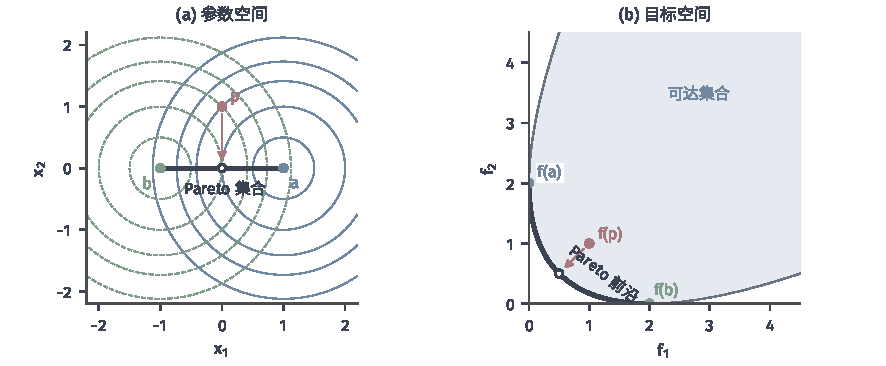
\includegraphics[width=150mm]{figures/03-optimization-evolution-and-signals/01-optimization/matplotlib/c7-pareto-set-front/figure.pdf}
  \caption{同一个双目标问题在两个空间中的样子，目标为式~\eqref{eq:opt-mmb-two-quadratics}。(a)参数平面上，实线圆是$f_1$的等值线，虚线圆是$f_2$的等值线；连接$\bm a,\bm b$的粗线段是Pareto集合。(b)目标平面上，阴影是可达集合$\bm f(\mathbb R^2)=\{(u,v):u+v\geq1+(u-v)^2/4\}$，粗曲线是Pareto前沿$((s-1)^2/2,(s+1)^2/2)$，$-1\leq s\leq1$。红点$\bm p=(0,1)$的像$(1,1)$在可达集合内部，箭头指向支配它的原点之像$(1/2,1/2)$。}
  \label{fig:opt-mmb-pareto-set-front}
\end{figure*}

一个候选不被支配，只说明“没有免费的改进”，并不说明它应当被采用。前沿上的$A$与$D$都是Pareto最优点，却代表截然不同的部署方案。所以多目标问题的输出可以是整个前沿的近似，也可以是按某种偏好选出的一点；下面两小节讨论后者如何确定。

\paragraph{Pareto点何时存在}
Pareto点不会自动存在。取$C=(0,1]$与$f_1(x)=f_2(x)=x$，任意$x$都被更小的$x/2$支配，Pareto集合是空集。缺口出在$C$不是闭集：两个指标共同的下确界$0$不可达。下面的结论用一个严格正权的标量目标把存在性归结为第~\ref{chap:optimization}章的Weierstrass型结论：非空紧集上的连续函数达到最小值。

\begin{theorem}[Pareto点的存在]
\label{thm:opt-mmb-pareto-existence}
设$C$非空紧，$f_1,\dots,f_m$在$C$上连续。则对任意满足$\alpha_i>0$的权重，函数$\sum_{i=1}^m\alpha_if_i$在$C$上达到最小值，且每个最小点都是Pareto最优点。特别地，Pareto集合非空。
\end{theorem}

\begin{proof}
连续函数的正系数线性组合仍连续，非空紧集上的连续函数达到最小值，所以最小点$\bm x^\star$存在。若某个$\bm u\in C$支配$\bm x^\star$，则$\alpha_if_i(\bm u)\leq\alpha_if_i(\bm x^\star)$对所有$i$成立，且对使$f_i(\bm u)<f_i(\bm x^\star)$的那个$i$，由$\alpha_i>0$得到严格不等式。逐项相加得$\sum_i\alpha_if_i(\bm u)<\sum_i\alpha_if_i(\bm x^\star)$，与$\bm x^\star$是最小点矛盾。
\end{proof}

证明中两个条件分工明确：紧性与连续性负责“最小点存在”，权重严格为正负责“最小点不被支配”。有限候选集总是紧的，所以式~\eqref{eq:opt-mmb-six-candidates}的任何正权组合都会选出$A,B,C,D$中的某一个。不过下一小节会看到，“选出的总是Pareto点”并不意味着“每个Pareto点都能被选出”。

\subsection{加权和法}
\label{sec:opt-mmb-weighted-sum}

\paragraph{用权重表达偏好}
最直接的偏好表达是给每个指标一个价格。取权重$\bm\alpha$属于概率单纯形$\Delta_m=\{\bm\alpha\in\mathbb R^m:\alpha_i\geq0,\ \sum_i\alpha_i=1\}$，求解
\begin{equation}
\label{eq:opt-mmb-weighted-sum}
\min_{\bm x\in C}\ \sum_{i=1}^m\alpha_if_i(\bm x).
\end{equation}
这样做的方法称为\term{加权和法}（weighted-sum method），它是把向量目标化为标量的\term{标量化}（scalarization）中最简单的一种。化成标量后，前面各章的方法可以直接使用：目标光滑时用第~\ref{chap:opt-smooth}章的梯度法，带约束时用第~\ref{chap:constrained-optimization}章的方法。

权重的数值本身没有绝对含义，它和指标的单位绑定在一起。若把延迟从毫秒改成秒，$f_1$的数值缩小为原来的千分之一，同一个$\alpha_1$代表的偏好就完全变了。实际使用时常先把每个指标除以一个参考尺度（例如它在候选中的取值范围），再讨论权重。无论权重怎样设定，求解后都应报告每个原始指标，而不是只报告加权值：加权值$2.25$本身无法告诉部署者延迟和误差各是多少。

\paragraph{加权和最小点的Pareto性质}
定理~\ref{thm:opt-mmb-pareto-existence}的证明已经说明正权最小点不被支配。允许某些权重为零时，结论要减弱。

\begin{theorem}[加权和最小点的性质]
\label{thm:opt-mmb-weighted-sum}
设$\bm\alpha\in\Delta_m$，$\bm x^\star$是问题~\eqref{eq:opt-mmb-weighted-sum}的全局最小点。若所有$\alpha_i>0$，则$\bm x^\star$是Pareto最优点；一般情形下，$\bm x^\star$是弱Pareto最优点。
\end{theorem}

\begin{proof}
第一部分的论证与定理~\ref{thm:opt-mmb-pareto-existence}相同。对一般的$\bm\alpha\in\Delta_m$，若有$\bm u\in C$使$f_i(\bm u)<f_i(\bm x^\star)$对所有$i$成立，则由$\alpha_i\geq0$且至少一个$\alpha_i>0$（权重之和为$1$），得$\sum_i\alpha_if_i(\bm u)<\sum_i\alpha_if_i(\bm x^\star)$，矛盾。
\end{proof}

零权确实会带来弱Pareto点。在有限例中取$\bm\alpha=(0,1)$，加权值就是误差$f_2$，$D$与$F$同时达到最小值$1$，而$F$被$D$支配。此时应在加权和的最小点中再剔除被支配者。

\paragraph{加权和只找到凸包上的点}
加权和的几何含义可以在目标平面上看清。固定$\bm\alpha=(\alpha,1-\alpha)$，满足$\alpha u+(1-\alpha)v=c$的点$(u,v)$构成法向为$(\alpha,1-\alpha)$的直线；最小化加权值，就是把这条直线从左下方向右上方平移，直到它第一次碰到可达集合。碰到的位置总在可达集合的“左下凸包”上。前沿若向右上方凹进去一块，任何方向的直线都会先碰到凹陷两侧的点，凹陷内部的点永远不会被选中。

在有限例中计算得
\[
\begin{aligned}
&A:\ 5-4\alpha,\qquad B:\ 2.5-0.5\alpha,\qquad C:\ 2.2+1.3\alpha,\\
&D:\ 1+4\alpha,\qquad E:\ 4,\qquad F:\ 1+5\alpha.
\end{aligned}
\]
$C$不劣于$B$要求$2.2+1.3\alpha\leq2.5-0.5\alpha$，即$\alpha\leq1/6$；$C$不劣于$D$要求$2.2+1.3\alpha\leq1+4\alpha$，即$\alpha\geq4/9$。两个条件不能同时成立，所以无论权重如何，$C$都不会被加权和选中，尽管它是Pareto最优点。几何上，$C$位于连接$B,D$的线段上方：线段在$f_1=3.5$处的高度是$2.5-1.5\times\frac{1.5}{3}=1.75<2.2$。图~\ref{fig:opt-mmb-weighted-sum}把这一现象画在连续前沿和有限候选两个场景中。

\begin{figure*}[!htbp]
  \centering
  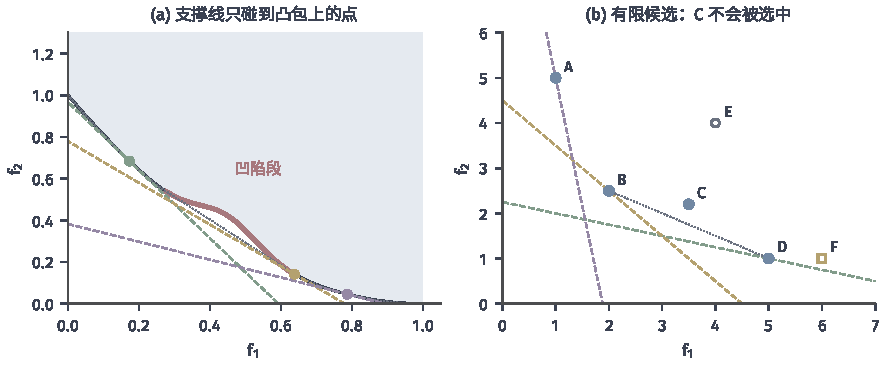
\includegraphics[width=150mm]{figures/03-optimization-evolution-and-signals/01-optimization/matplotlib/c7-weighted-sum/figure.pdf}
  \caption{加权和的支撑线。(a)示意的连续前沿$v=(1-u)^2+0.12\exp(-((u-0.45)/0.12)^2)$，$0\leq u\leq1$（严格递减，每点都是Pareto点），阴影为其右上方的可达区域；三条虚线是$\alpha=0.62,0.5,0.3$时的最低加权等值线，切点分别落在前沿上。点线是前沿的下凸包，红色粗线标出不在凸包上的凹陷段（约$0.27<u<0.63$），没有任何权重能选中其中的点。(b)有限候选中$\alpha=0.85,0.5,0.2$的最低等值线分别经过$A,B,D$；$C$在点线$BD$上方，永远不会被选中。}
  \label{fig:opt-mmb-weighted-sum}
\end{figure*}

如果可达集合向右上方扩张后是凸的（例如$C$凸、各$f_i$凸时），凹陷不会出现。这时可以借助第~\ref{chap:constrained-optimization}章的凸集分离超平面说明：每个弱Pareto点都是某个$\bm\alpha\in\Delta_m$对应的加权和最小点。设$\bar{\bm y}=\bm f(\bar{\bm x})$是弱Pareto点的像，集合$\bm f(C)+\mathbb R^m_{\geq0}$凸，它与开凸集$\{\bm y:y_i<\bar y_i\ \forall i\}$不相交，对差集$\bigl(\bm f(C)+\mathbb R^m_{\geq0}\bigr)-\{\bm y:y_i<\bar y_i\ \forall i\}$这个不含原点的开凸集，用该章的点与闭凸集分离（原点在闭包边界上时，对趋于原点的外点分离再取法向量的极限）得到分离超平面；由于前一集合沿各坐标正方向无界，法向量可取为非负并归一化，这正是所需的权重。非凸问题没有这一保证，所以“扫遍权重即可描出前沿”只在凸情形下可靠。

\paragraph{权重变化与解的跳变}
即使不考虑凹陷，最小点也不必随权重连续移动。有限例中，$\alpha<1/3$时$D$最好，$1/3<\alpha<5/7$时$B$最好，$\alpha>5/7$时$A$最好；$\alpha=1/3$处$B$与$D$并列（加权值都是$7/3$），$\alpha=5/7$处$A$与$B$并列（都是$15/7$）。权重穿过这些临界值时，答案从一个候选跳到另一个，中间的方案没有机会出现。连续问题的前沿若含直线段，同样会在某个权重处出现整段并列的最小点。

\subsection{阈值约束法}
\label{sec:opt-mmb-epsilon-constraint}

\paragraph{把其余指标写成上限}
许多场合的偏好不是价格，而是硬性要求：延迟不能超过某个上限，在此前提下误差越小越好。把这种要求直接写成约束，就得到\term{阈值约束法}（epsilon-constraint method）：保留第$j$个指标作目标，其余指标给出上限$\tau_i$，
\begin{equation}
\label{eq:opt-mmb-epsilon-constraint}
\min_{\bm x\in C}\ f_j(\bm x)\qquad\text{s.t.}\quad f_i(\bm x)\leq\tau_i,\quad i\neq j.
\end{equation}
这是一个普通的约束优化问题，第~\ref{chap:constrained-optimization}章的可行性判断、乘子与求解方法都可以接入。阈值的位置决定约束的状态：阈值过低时问题不可行，应当报告“不存在满足要求的方案”，而不是返回一个违背约束的点；阈值恰好卡住最优解时约束激活，相应乘子度量放宽一单位上限能换来的目标改善；阈值很宽松时约束不起作用，问题退化为只优化$f_j$。

\paragraph{阈值法能到达每个Pareto点}
阈值法与加权和最大的不同在于，它不需要支撑直线，因此能进入凹陷。

\begin{theorem}[阈值约束问题的解]
\label{thm:opt-mmb-epsilon-constraint}
固定$j$与阈值$\tau_i$（$i\neq j$）。
\begin{enumerate}
  \item 问题~\eqref{eq:opt-mmb-epsilon-constraint}的每个全局最小点都是弱Pareto最优点；若全局最小点唯一，它是Pareto最优点。
  \item 反过来，若$\bar{\bm x}$是Pareto最优点，取$\tau_i=f_i(\bar{\bm x})$（$i\neq j$），则$\bar{\bm x}$是问题~\eqref{eq:opt-mmb-epsilon-constraint}的全局最小点。
\end{enumerate}
\end{theorem}

\begin{proof}
(1)设$\hat{\bm x}$是全局最小点。若某个$\bm u\in C$使所有$f_i(\bm u)<f_i(\hat{\bm x})$，则$f_i(\bm u)<f_i(\hat{\bm x})\leq\tau_i$说明$\bm u$可行，而$f_j(\bm u)<f_j(\hat{\bm x})$与最优性矛盾，所以$\hat{\bm x}$弱Pareto最优。若$\hat{\bm x}$是唯一最小点而$\bm u$支配它，则$f_i(\bm u)\leq f_i(\hat{\bm x})\leq\tau_i$说明$\bm u$可行，$f_j(\bm u)\leq f_j(\hat{\bm x})$说明$\bm u$也是最小点，于是$\bm u=\hat{\bm x}$，这与“至少一项严格更小”矛盾。

(2)$\bar{\bm x}$满足$f_i(\bar{\bm x})\leq\tau_i$，是可行点。若某个可行点$\bm u$使$f_j(\bm u)<f_j(\bar{\bm x})$，再由可行性$f_i(\bm u)\leq\tau_i=f_i(\bar{\bm x})$（$i\neq j$），$\bm u$支配$\bar{\bm x}$，与Pareto最优矛盾。
\end{proof}

第二部分不需要任何凸性：只要把阈值设在某个Pareto点的指标值上，那个点就是阈值问题的解。图~\ref{fig:opt-mmb-threshold}左栏中，竖直的阈值线$f_1\leq\tau$从左向右扫过时，选出的点沿整条前沿移动，包括加权和无法到达的凹陷段。代价是：阈值问题的解可能不唯一，此时只能保证弱Pareto性，需要在并列的最小点中再剔除被支配者。

\paragraph{有限例上的预算与价格}
在有限例上以延迟为预算、以误差为目标，计算$\min\{f_2:f_1\leq\tau\}$。$\tau<1$时不可行；$1\leq\tau<2$时只有$A$可行；$2\leq\tau<3.5$时选$B$；$3.5\leq\tau<5$时选$C$；$\tau\geq5$时选$D$，而$\tau\geq6$后$D$与$F$并列，$F$只是弱Pareto点，应剔除。与加权和的结果对照（图~\ref{fig:opt-mmb-threshold}右栏），两种方法在同一个候选集上覆盖的答案不同：预算法能返回$C$，价格法永远不能。两者也都会跳变：预算每跨过一个候选的延迟值，答案就离散地换成另一个候选。

\begin{figure*}[!htbp]
  \centering
  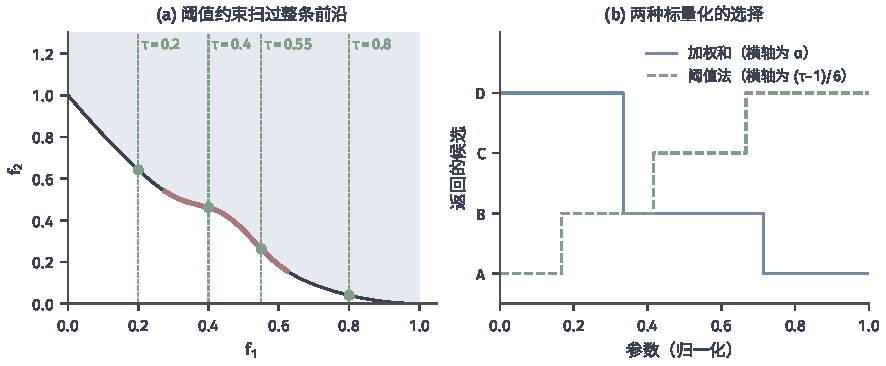
\includegraphics[width=150mm]{figures/03-optimization-evolution-and-signals/01-optimization/matplotlib/c7-threshold/figure.pdf}
  \caption{阈值约束法。(a)与图~\ref{fig:opt-mmb-weighted-sum}(a)相同的前沿，四条竖虚线是延迟上限$\tau=0.2,0.4,0.55,0.8$，圆点是$\min\{f_2:f_1\leq\tau\}$的解；后两个解位于红色凹陷段内，加权和选不到它们。(b)有限例中两种标量化返回的候选：实线是加权和随$\alpha\in[0,1]$的选择，虚线是阈值法随$\tau\in[1,7]$（横轴换算为$(\tau-1)/6$）的选择；并列时按字母顺序取第一个。只有阈值法会返回$C$。}
  \label{fig:opt-mmb-threshold}
\end{figure*}

码率与失真的权衡是同一结构的常见例子：编码方案的码率越低越好，失真也越低越好。给定有限个编码配置时，“码率不超过预算时失真最小”就是阈值问题，“失真加上码率乘以价格最小”就是加权和，二者覆盖的配置可以不同。概率意义下的率失真函数还需要信源分布与信息量的定义，它在\BookChapterRef{chap:information-theory-and-statistical-geometry}{卷四“概率分布的分析与优化”章}中建立，这里只把有限配置当作普通的双指标候选。

\subsection{共同下降方向}
\label{sec:opt-mmb-common-descent}

加权和与阈值法都先把偏好固定下来，再求解一个标量问题。另一种做法是不预设偏好，从当前点出发寻找让所有指标同时下降的方向，直到再也找不到为止。这在指标可微、维数很高（例如多任务学习中共享参数的若干损失）时很自然：每一步只需计算各指标的梯度。

\paragraph{梯度凸包中的最小范数元}
设$C=\mathbb R^d$，各$f_i$在$\bm x$处可微。方向$\bm d$若满足$\langle\nabla f_i(\bm x),\bm d\rangle<0$对所有$i$成立，则沿$\bm d$走足够小的一步，每个指标都严格下降，称它为严格的\term{共同下降方向}（common descent direction）。怎样找到这样的方向？考虑梯度的凸包$\operatorname{conv}\{\nabla f_1(\bm x),\dots,\nabla f_m(\bm x)\}$中离原点最近的点
\begin{equation}
\label{eq:opt-mmb-min-norm}
\bar{\bm g}=\sum_{i=1}^m\alpha_i^\star\nabla f_i(\bm x),\quad
\bm\alpha^\star\in\argmin_{\bm\alpha\in\Delta_m}\ \frac12\Bigl\lVert\sum_{i=1}^m\alpha_i\nabla f_i(\bm x)\Bigr\rVert_2^2.
\end{equation}
权重子问题是单纯形上的凸二次规划，变量个数只有$m$。凸包是非空紧凸集，$\bar{\bm g}$就是原点在它上面的投影，因而唯一（权重$\bm\alpha^\star$未必唯一）。两个指标时子问题有闭式解：记$\bm g_1,\bm g_2$为两个梯度，$\bm g_1\neq\bm g_2$时
\[
\alpha_1^\star=\min\Bigl\{1,\max\Bigl\{0,\frac{\langle\bm g_2,\bm g_2-\bm g_1\rangle}{\lVert\bm g_1-\bm g_2\rVert_2^2}\Bigr\}\Bigr\},
\]
这是对$\lVert\bm g_2+\alpha(\bm g_1-\bm g_2)\rVert_2^2$关于$\alpha$求最小再截断到$[0,1]$的结果。

\begin{lemma}[最小范数元给出共同下降]
\label{lem:opt-mmb-min-norm-descent}
若$\bar{\bm g}\neq\bm 0$，则$\langle\nabla f_i(\bm x),-\bar{\bm g}\rangle\leq-\lVert\bar{\bm g}\rVert_2^2$对所有$i$成立。
\end{lemma}

\begin{proof}
第~\ref{chap:opt-nonsmooth}章建立的投影刻画是：$\bm p$是点$\bm z$在非空闭凸集$K$上的投影，当且仅当$\bm p\in K$且$\langle\bm z-\bm p,\bm v-\bm p\rangle\leq0$对所有$\bm v\in K$成立。取$K$为梯度凸包，$\bm z=\bm 0$，$\bm p=\bar{\bm g}$，$\bm v=\nabla f_i(\bm x)$，得$\langle-\bar{\bm g},\nabla f_i(\bm x)-\bar{\bm g}\rangle\leq0$，整理即为结论。
\end{proof}

\begin{theorem}[一阶共同下降的判据]
\label{thm:opt-mmb-pareto-stationary}
设$C=\mathbb R^d$，各$f_i$在$\bm x$处可微。在$\bm x$处不存在严格的共同下降方向，当且仅当存在$\bm\alpha\in\Delta_m$使$\sum_i\alpha_i\nabla f_i(\bm x)=\bm 0$，即$\bar{\bm g}=\bm 0$。
\end{theorem}

\begin{proof}
若$\sum_i\alpha_i\nabla f_i(\bm x)=\bm 0$而某个$\bm d$使每个$\langle\nabla f_i(\bm x),\bm d\rangle<0$，乘以非负且不全为零的$\alpha_i$后相加得$0=\langle\bm 0,\bm d\rangle<0$，矛盾。反过来，若$\bm 0$不在梯度凸包中，则$\bar{\bm g}\neq\bm 0$，由引理~\ref{lem:opt-mmb-min-norm-descent}，$-\bar{\bm g}$就是严格的共同下降方向。
\end{proof}

满足$\bar{\bm g}=\bm 0$的点常称为Pareto驻点。$m=1$时凸包只有一个梯度，判据退回到$\nabla f_1(\bm x)=\bm 0$。

\paragraph{一个可以手算的例子}
回到式~\eqref{eq:opt-mmb-two-quadratics}的两个二次指标，在$\bm p=(0,1)$处$\nabla f_1(\bm p)=\bm p-\bm a=(-1,1)$，$\nabla f_2(\bm p)=\bm p-\bm b=(1,1)$。闭式解给出$\alpha_1^\star=\langle(1,1),(2,0)\rangle/4=1/2$，$\bar{\bm g}=(0,1)$。两梯度与$-\bar{\bm g}=(0,-1)$的内积都是$-1=-\lVert\bar{\bm g}\rVert_2^2$，与引理一致。沿$-\bar{\bm g}$走步长$1$到达原点，$f_1$与$f_2$都从$1$降到$1/2$；原点处两梯度为$(-1,0)$与$(1,0)$，零向量是它们的平均，不再有共同下降方向。图~\ref{fig:opt-mmb-common-descent}左栏画出了这一步：两条梯度箭头张成的线段上离$\bm p$最近的点决定$\bar{\bm g}$，而所有使两项同时下降的方向组成一个开锥$\{\bm d:d_2<-|d_1|\}$。

\begin{figure*}[!htbp]
  \centering
  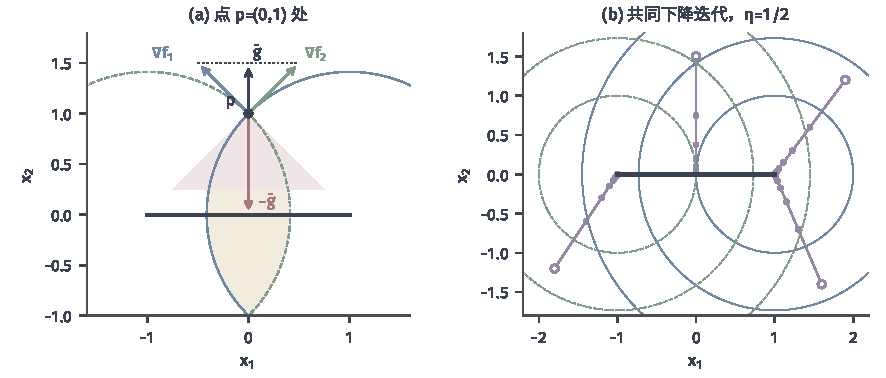
\includegraphics[width=150mm]{figures/03-optimization-evolution-and-signals/01-optimization/matplotlib/c7-common-descent/figure.pdf}
  \caption{共同下降方向，目标为式~\eqref{eq:opt-mmb-two-quadratics}。(a)在$\bm p=(0,1)$处，两条梯度箭头（按$1/2$缩放）之间的点线是梯度凸包，其中最短的向量是$\bar{\bm g}=(0,1)$；红色锥是使两项都严格下降的方向，$-\bar{\bm g}$位于锥的中轴。两段圆弧是过$\bm p$的两条等值线，黄色透镜区域中的点使两项都比在$\bm p$处小。(b)从四个起点出发、步长$\eta=1/2$的共同下降迭代，每条轨迹都停在Pareto集合（粗线段）上，停在哪一点取决于起点。}
  \label{fig:opt-mmb-common-descent}
\end{figure*}

\paragraph{步长与停止}
引理~\ref{lem:opt-mmb-min-norm-descent}只保证方向正确，步长仍要控制。若每个$f_i$的梯度是$L_i$-Lipschitz的（第~\ref{chap:opt-smooth}章的$L$-光滑条件），对每个$i$用二次上界得
\[
f_i(\bm x-\eta\bar{\bm g})\leq f_i(\bm x)-\eta\lVert\bar{\bm g}\rVert_2^2+\frac{L_i\eta^2}{2}\lVert\bar{\bm g}\rVert_2^2,
\]
所以$0<\eta\leq1/\max_iL_i$时每个指标至少下降$\frac{\eta}{2}\lVert\bar{\bm g}\rVert_2^2$。光滑常数未知时，像第~\ref{chap:opt-smooth}章的Armijo回溯那样缩小步长，但接受条件必须对每个指标分别检查。完整的一轮如算法~\ref{alg:opt-mmb-mgda}所示。

\begin{algorithm}[带回溯的共同下降法]
\label{alg:opt-mmb-mgda}
\begin{algorithmic}[1]
\Require 初始点$\bm x^{(0)}$，初始步长$\bar\eta>0$，缩步因子$\rho\in(0,1)$，充分下降常数$c\in(0,1)$，容差$\varepsilon>0$
\Ensure 近似Pareto驻点$\bm x^{(t)}$及各指标值
\For{$t=0,1,2,\dots$}
  \State 计算$m$个梯度$\nabla f_i(\bm x^{(t)})$，解单纯形上的二次规划~\eqref{eq:opt-mmb-min-norm}得$\bar{\bm g}^{(t)}$
  \If{$\lVert\bar{\bm g}^{(t)}\rVert_2\leq\varepsilon$}
    \State \Return $\bm x^{(t)}$与$f_1(\bm x^{(t)}),\dots,f_m(\bm x^{(t)})$
  \EndIf
  \State $\eta\gets\bar\eta$
  \While{存在$i$使$f_i(\bm x^{(t)}-\eta\bar{\bm g}^{(t)})>f_i(\bm x^{(t)})-c\,\eta\lVert\bar{\bm g}^{(t)}\rVert_2^2$}
    \State $\eta\gets\rho\eta$
  \EndWhile
  \State $\bm x^{(t+1)}\gets\bm x^{(t)}-\eta\bar{\bm g}^{(t)}$
\EndFor
\end{algorithmic}
\end{algorithm}

在$L_i$-光滑条件下，上面的二次上界说明$\eta\leq2(1-c)/\max_iL_i$时接受条件对所有$i$成立，所以回溯有限步结束。每轮的代价是$m$次梯度计算、一个$m$维二次规划（形成Gram矩阵$\langle\nabla f_i,\nabla f_k\rangle$需$O(m^2d)$次运算），以及每次试探步上$m$个指标的求值。图~\ref{fig:opt-mmb-common-descent}右栏显示，不同起点停在前沿的不同位置：这一方法只保证“不再能同时改善”，不替我们决定停在哪一种取舍上。

\paragraph{一阶判据的边界}
定理~\ref{thm:opt-mmb-pareto-stationary}是一阶条件，它排除的只是一阶意义下的共同改善，不能代替Pareto最优。取$m=2$、$d=1$、$f_1(x)=f_2(x)=-x^2$，在$x=0$处两梯度都为零，判据成立，而$0$是两个指标共同的极大点，任何$x\neq0$都支配它。再取$f_1(x)=0$、$f_2(x)=x^2$，在$x=1$处$\nabla f_1=0$，取$\bm\alpha=(1,0)$即得零组合，但$x=1$被$x=0$支配。第二个例子中，零组合把全部权重压在一个不随$x$变化的指标上，正对应定理~\ref{thm:opt-mmb-weighted-sum}中零权只保弱Pareto的情形。有约束时，方向还必须保持可行，梯度凸包判据要换成只在可行方向上检查，第~\ref{chap:constrained-optimization}章的可行方向与乘子工具在这里同样需要。

增加凸性后，一阶判据可以加强为全局结论。设各$f_i$在$\mathbb R^d$上凸且可微，$\sum_i\alpha_i\nabla f_i(\bar{\bm x})=\bm 0$，$\bm\alpha\in\Delta_m$。则$\sum_i\alpha_if_i$是凸函数且在$\bar{\bm x}$处梯度为零，由第~\ref{chap:optimization}章的凸函数一阶条件，$\bar{\bm x}$是它的全局最小点；再由定理~\ref{thm:opt-mmb-weighted-sum}，$\bar{\bm x}$是弱Pareto最优点，若所有$\alpha_i>0$则是Pareto最优点。式~\eqref{eq:opt-mmb-two-quadratics}中原点对应$\bm\alpha=(1/2,1/2)$，因此它确实是Pareto最优点，与直接分析一致。
